\section{Auswertung}
\label{sec:Auswertung}

Die Graphen werden sowohl mit Matplotlib \cite{matplotlib} als auch NumPy \cite{numpy} erstellt. Die Fehlerrechnung wird mithilfe von Uncertainties \cite{uncertainties} durchgeführt. Der Fehler der Impulsrate $N$ unterliegt der Poisson-Verteilung und berechnet sich durch $\sigma_.N=\sqrt{N}$. Bei der Bestimmung der Halbwertszeiten wird die gemessene Impulsrate um die bei der Nulleffektmessung bestimmte Nullrate von $N_0=\SI{0.25}{\becquerel}$ korrigiert.

\subsection{Vanadium}

Es wird die Halbwertszeit und die Zerfallskurve von Vanadium ($^{52}_{23}.V$) bestimmt.
Eine lineare Ausgleichsrechnung der Form \[\ln(N_.{V_{52}}(t))=-\lambda_.{V_{52}} t+\ln(N_.{0,V_{52}})\] ergibt mit den Werten aus Tabelle \ref{tab:tabVanadium}:
\begin{align*}
\lambda_.{V_{52}}	&= \SI{2.9(2)e-3}{1\per\second}\text{,}\\
N_.{0,V_{52}} 		&= \SI{1.5(2)}{\becquerel}\text{.}
\end{align*}
Die Halbwertszeit $\tau$ ergibt sich mit Formel \eqref{eq:T} zu:
\begin{equation*}
\tau_.{V_{52}} = \SI{241(20)}{\second}\text{.}
\end{equation*}
Der Fehler $\sigma_{\tau}$ berechnet sich mit:
\begin{equation}
\sigma_{\tau} = \frac{\sigma_{\lambda}}{\lambda^2}\label{eq:sigma_tau}
\end{equation}
Dabei ist $\sigma_{\lambda}$ der Fehler von $\lambda$. Die Messwerte aus Tabelle \ref{tab:tabVanadium} sind in den Graphen \ref{fig:VanadiumLog} und \ref{fig:Vanadium} gegeneinander aufgetragen.

\begin{table}
	\centering
	\caption{Die Messwerte von Vanadium für die Zeit t, die Impulsrate $N_.V$ und deren Fehler, sowie die berechneten logarithmierten Werte.}
	\label{tab:tabVanadium}
	\sisetup{table-format=1.2}
	\begin{tabular}{S[table-format=3.0]S[table-format=1.1]S[table-format=1.1]S[table-format=1.2]S[table-format=1.2]S[table-format=1.2]}
		\toprule
		{$t/\si{\second}$} & {$N_.V/\si{\becquerel}$} & {$\sigma_{N_.V}/\si{\becquerel}$} & {$\ln\left(N_.V/\si{\becquerel}\right)$} & {$\ln\left(\frac{N_.V+\sigma_{N_.V}}{N}\right)$} & {$\ln\left(\frac{N_.V}{N_.V-\sigma_{N_.V}}\right)$} \\
		\midrule
		 30 & 2.1 & 0.3 & 0.75 & 0.12 & 0.13 \\
		 60 & 1.2 & 0.2 & 0.17 & 0.16 & 0.18 \\
		 90 & 0.9 & 0.2 & -0.12 & 0.18 & 0.22 \\
		120 & 1.1 & 0.2 & 0.11 & 0.16 & 0.19 \\
		150 & 1.0 & 0.2 & 0.02 & 0.17 & 0.20 \\
		180 & 0.8 & 0.2 & -0.20 & 0.18 & 0.23 \\
		210 & 0.9 & 0.2 & -0.08 & 0.17 & 0.21 \\
		240 & 0.6 & 0.1 & -0.54 & 0.21 & 0.27 \\
		270 & 0.7 & 0.2 & -0.33 & 0.20 & 0.24 \\
		300 & 0.7 & 0.2 & -0.38 & 0.20 & 0.25 \\
		330 & 0.7 & 0.1 & -0.43 & 0.20 & 0.26 \\
		360 & 0.6 & 0.1 & -0.48 & 0.21 & 0.26 \\
		390 & 0.5 & 0.1 & -0.66 & 0.23 & 0.29 \\
		420 & 0.3 & 0.1 & -1.14 & 0.28 & 0.39 \\
		450 & 0.6 & 0.1 & -0.54 & 0.21 & 0.27 \\
		480 & 0.4 & 0.1 & -0.87 & 0.25 & 0.33 \\
		510 & 0.1 & 0.1 & -2.13 & 0.42 & 0.75 \\
		540 & 0.3 & 0.1 & -1.14 & 0.28 & 0.39 \\
		570 & 0.2 & 0.1 & -1.52 & 0.33 & 0.49 \\
		600 & 0.2 & 0.1 & -1.52 & 0.33 & 0.49 \\
		630 & 0.2 & 0.1 & -1.88 & 0.38 & 0.63 \\
		690 & 0.4 & 0.1 & -1.04 & 0.27 & 0.37 \\
		720 & 0.2 & 0.1 & -1.88 & 0.38 & 0.63 \\
		750 & 0.3 & 0.1 & -1.38 & 0.31 & 0.45 \\
		780 & 0.2 & 0.1 & -1.68 & 0.35 & 0.55 \\
		810 & 0.1 & 0.1 & -2.13 & 0.42 & 0.75 \\
		840 & 0.2 & 0.1 & -1.88 & 0.38 & 0.63 \\
		870 & 0.1 & 0.1 & -2.46 & 0.49 & 0.98 \\
		900 & 0.2 & 0.1 & -1.68 & 0.35 & 0.55 \\
		\bottomrule
	\end{tabular}

	\label{tab:tabVanadium}
\end{table}

\begin{figure}
	\centering
	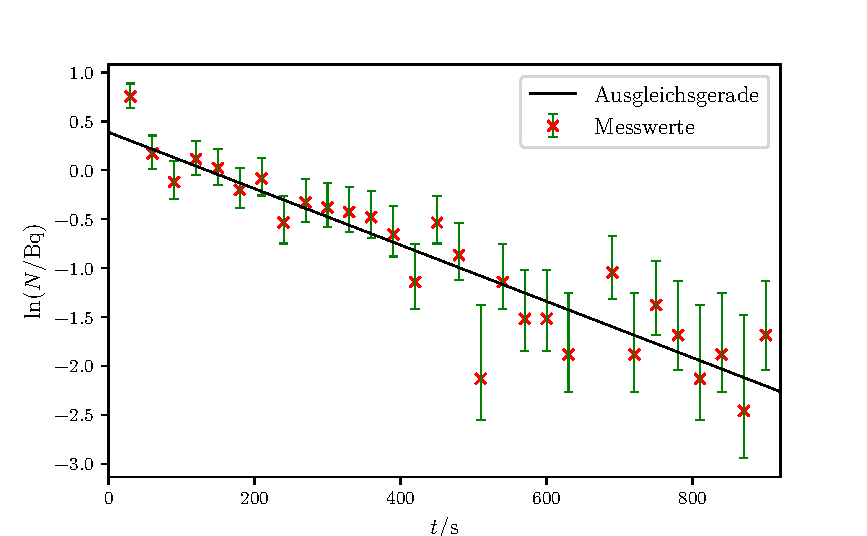
\includegraphics[width=\linewidth-50pt,height=\textheight-50pt,keepaspectratio]{content/images/VanadiumLog.pdf}
	\caption{Die logarithmische Impulsrate $N_.V$ von Vanadium in Abhängigkeit von der Zeit $t$.}
	\label{fig:VanadiumLog}
\end{figure}

\begin{figure}
	\centering
	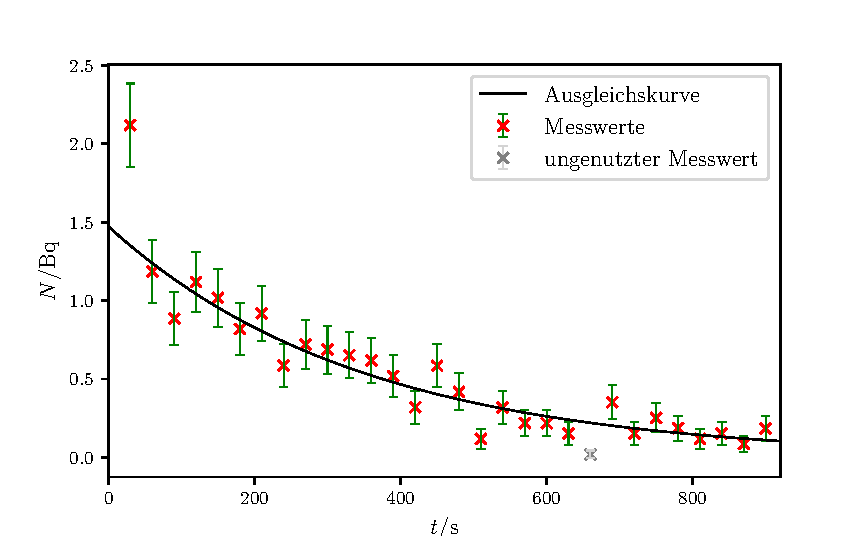
\includegraphics[width=\linewidth-50pt,height=\textheight-50pt,keepaspectratio]{content/images/Vanadium.pdf}
	\caption{Die Impulsrate $N_.V$ von Vanadium in Abhängigkeit von der Zeit $t$.}
	\label{fig:Vanadium}
\end{figure}


\subsection{Rhodium}

Es werden die Halbwertszeiten und die Zerfallskurven von Rhodium ($^{104}_{45}.{Rh}$ und $^{104i}_{45}.{Rh}$) bestimmt.
Eine lineare Ausgleichsrechnung der Form 
\begin{equation}
\ln(N_.{Rh_.{104i}}(t))=-\lambda_.{Rh_.{104i}} t+\ln(N_.{0,Rh_.{104i}})\label{eq:Ausgleich2}
\end{equation}
für $t\geq 250$ ergibt mit den Werten aus Tabelle \ref{tab:tabRhodium}
\begin{align*}
\lambda_.{Rh_.{104i}} 	&= \SI{2.6(7)e-3}{1\per\second}\text{,}\\
N_.{0,Rh_.{104i}} 		&= \SI{5(1)}{\becquerel}\text{.}
\end{align*}
Hiermit lässt sich für $t\leq 190$ eine Ausgleichsrechnung der Form 
\begin{equation}
\ln(N_.{Rh_.{104}}(t))=\ln(N_.{Rh}-N_.{Rh_.{104i}}(t))=-\lambda_.{Rh_.{104}} t+\ln(N_.{0,Rh_.{104}})\label{eq:Ausgleich1}
\end{equation}
durchführen:
\begin{align*}
\lambda_.{Rh_.{104}} 	&= \SI{1.64(8)e-2}{1\per\second}\text{,}\\
N_.{0,Rh_.{104}} 		&= \SI{44(4)}{\becquerel}\text{.}
\end{align*}
Die Halbwertszeiten ergeben sich nach Formel \eqref{eq:T} zu:
\begin{align*}
\tau_.{Rh_.{104i}} 	&= \SI{260(70)}{\second}\text{,}\\
\tau_.{Rh_.{104}} &= \SI{42(2)}{\second}\text{.}
\end{align*}
Die Fehler berechnen sich nach Formel \eqref{eq:sigma_tau}. Die Messwerte aus Tabelle \ref{tab:tabRhodium} sind in den Graphen von \ref{fig:RhodiumLog1} bis \ref{fig:Rhodium} gegeneinander aufgetragen. Dabei berechnet sich $N(t)$ nach:
\begin{equation*}
N(t)=N_.{Rh_.{104}}(t)+N_.{Rh_.{104i}}(t)=N_.{0,Rh_.{104}}.e^{-\lambda_.{Rh_.{104}} t}+N_.{0,Rh_.{104i}}.e^{-\lambda_.{Rh_.{104i}} t}
\end{equation*}

\begin{table}
	\centering
	\caption{Die Messwerte von Rhodium für die Zeit $t$, die Impulsrate $N_.{Rh}$ und deren Fehler, sowie die berechneten logarithmierten Werte.}
	\label{tab:tabRhodium1}
	\sisetup{table-format=1.2}
	\begin{tabular}{S[table-format=3.0]S[table-format=1.1]S[table-format=1.1]S[table-format=1.2]S[table-format=1.2]S[table-format=1.2]}
		\toprule
		{$t/\si{\second}$} & {$N_.{Rh}/\si{\becquerel}$} & {$\sigma_{N_.{Rh}}/\si{\becquerel}$} & {$\ln\left(N_.{Rh}/\si{\becquerel}\right)$} & {$\left|\ln\left(\frac{N_.{Rh}+\sigma_{N_.{Rh}}}{N_.{Rh}}\right)\right|$} & {$\left|\ln\left(\frac{N_.{Rh}}{N_.{Rh}-\sigma_{N_.{Rh}}}\right)\right|$} \\
		\midrule
		 10 & 40.2 & 2.0 & 3.69 & 0.05 & 0.05 \\
		 20 & 40.7 & 2.0 & 3.71 & 0.05 & 0.05 \\
		 30 & 31.6 & 1.8 & 3.45 & 0.05 & 0.06 \\
		 40 & 29.2 & 1.7 & 3.37 & 0.06 & 0.06 \\
		 50 & 24.9 & 1.6 & 3.21 & 0.06 & 0.07 \\
		 60 & 20.2 & 1.4 & 3.00 & 0.07 & 0.07 \\
		 70 & 19.6 & 1.4 & 2.97 & 0.07 & 0.07 \\
		 80 & 17.3 & 1.3 & 2.85 & 0.07 & 0.08 \\
		 90 & 13.8 & 1.2 & 2.62 & 0.08 & 0.09 \\
		100 & 13.7 & 1.2 & 2.61 & 0.08 & 0.09 \\
		110 & 8.0 & 0.9 & 2.07 & 0.11 & 0.12 \\
		120 & 9.6 & 1.0 & 2.26 & 0.10 & 0.11 \\
		130 & 8.4 & 0.9 & 2.12 & 0.10 & 0.12 \\
		140 & 7.7 & 0.9 & 2.03 & 0.11 & 0.12 \\
		150 & 8.0 & 0.9 & 2.07 & 0.11 & 0.12 \\
		160 & 7.1 & 0.8 & 1.95 & 0.11 & 0.13 \\
		170 & 5.3 & 0.7 & 1.66 & 0.13 & 0.15 \\
		180 & 5.3 & 0.7 & 1.66 & 0.13 & 0.15 \\
		190 & 6.3 & 0.8 & 1.83 & 0.12 & 0.14 \\
		200 & 4.5 & 0.7 & 1.49 & 0.14 & 0.16 \\
		210 & 3.5 & 0.6 & 1.24 & 0.16 & 0.19 \\
		220 & 2.7 & 0.5 & 0.98 & 0.18 & 0.22 \\
		230 & 2.2 & 0.5 & 0.77 & 0.20 & 0.24 \\
		240 & 5.2 & 0.7 & 1.64 & 0.13 & 0.15 \\
		250 & 3.1 & 0.6 & 1.12 & 0.17 & 0.20 \\
		260 & 3.0 & 0.5 & 1.08 & 0.17 & 0.20 \\
		270 & 2.9 & 0.5 & 1.05 & 0.17 & 0.21 \\
		280 & 2.6 & 0.5 & 0.94 & 0.18 & 0.22 \\
		290 & 2.3 & 0.5 & 0.81 & 0.19 & 0.24 \\
		\bottomrule
	\end{tabular}

	\label{tab:tabRhodium}
\end{table}

\begin{table}
	\centering
	\label{tab:tabRhodium2}
	\sisetup{table-format=1.2}
	\begin{tabular}{S[table-format=3.0]S[table-format=1.1]S[table-format=1.1]S[table-format=1.2]S[table-format=1.2]S[table-format=1.2]}
		\toprule
		{$t/\si{\second}$} & {$N_.{Rh}/\si{\becquerel}$} & {$\sigma_{N_.{Rh}}/\si{\becquerel}$} & {$\ln\left(N_.{Rh}/\si{\becquerel}\right)$} & {$\left|\ln\left(\frac{N_.{Rh}+\sigma_{N_.{Rh}}}{N_.{Rh}}\right)\right|$} & {$\left|\ln\left(\frac{N_.{Rh}}{N_.{Rh}-\sigma_{N_.{Rh}}}\right)\right|$} \\
		\midrule
		300 & 2.4 & 0.5 & 0.86 & 0.19 & 0.23 \\
		310 & 2.6 & 0.5 & 0.94 & 0.18 & 0.22 \\
		320 & 1.5 & 0.4 & 0.37 & 0.23 & 0.30 \\
		330 & 2.1 & 0.5 & 0.72 & 0.20 & 0.25 \\
		340 & 2.1 & 0.5 & 0.72 & 0.20 & 0.25 \\
		350 & 1.8 & 0.4 & 0.56 & 0.21 & 0.27 \\
		360 & 1.6 & 0.4 & 0.44 & 0.23 & 0.29 \\
		370 & 1.9 & 0.4 & 0.62 & 0.21 & 0.26 \\
		380 & 2.1 & 0.5 & 0.72 & 0.20 & 0.25 \\
		390 & 2.0 & 0.4 & 0.67 & 0.20 & 0.26 \\
		400 & 1.9 & 0.4 & 0.62 & 0.21 & 0.26 \\
		410 & 1.6 & 0.4 & 0.44 & 0.23 & 0.29 \\
		420 & 1.5 & 0.4 & 0.37 & 0.23 & 0.30 \\
		430 & 1.8 & 0.4 & 0.56 & 0.21 & 0.27 \\
		440 & 2.1 & 0.5 & 0.72 & 0.20 & 0.25 \\
		\bottomrule
	\end{tabular}

\end{table}

\begin{figure}
	\centering
	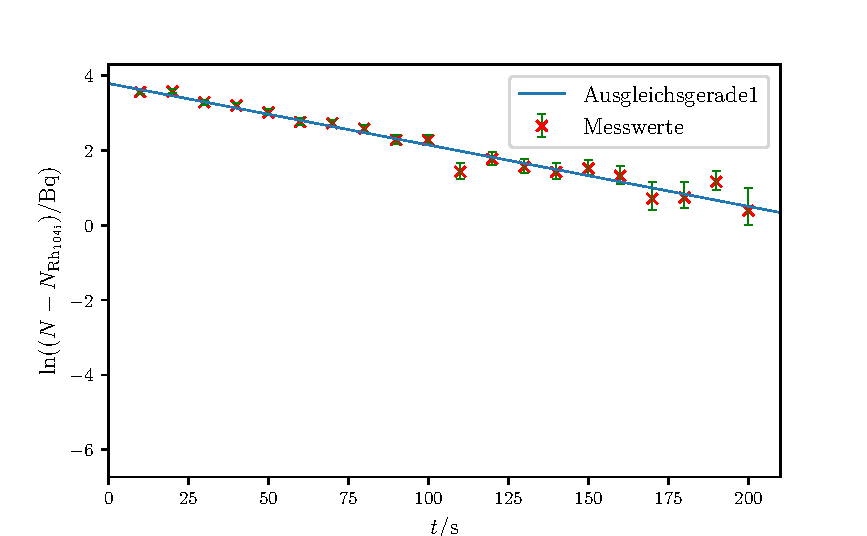
\includegraphics[width=\linewidth-50pt,height=\textheight-50pt,keepaspectratio]{content/images/RhodiumLog1.pdf}
	\caption{Die logarithmische Impulsrate $N_.{Rh_.{104}}$ von $^{104}_{45}.{Rh}$ in Abhängigkeit von der Zeit $t$. Die Ausgleichsgerade ist nach Formel \eqref{eq:Ausgleich1} berechnet.}
	\label{fig:RhodiumLog1}
\end{figure}

\begin{figure}
	\centering
	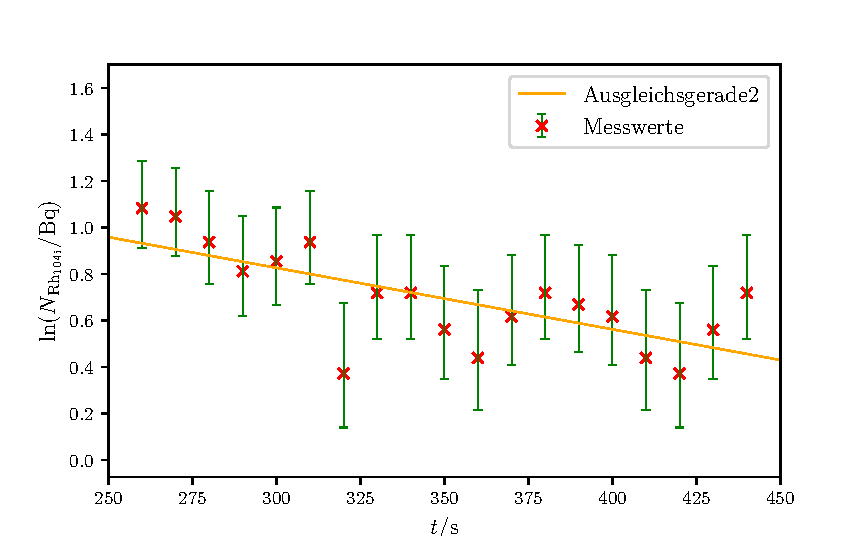
\includegraphics[width=\linewidth-50pt,height=\textheight-50pt,keepaspectratio]{content/images/RhodiumLog2.pdf}
	\caption{Die logarithmische Impulsrate $N_.{Rh_.{104i}}$ von $^{104i}_{45}.{Rh}$ in Abhängigkeit von der Zeit $t$. Die Ausgleichsgerade ist nach Formel \eqref{eq:Ausgleich2} berechnet.}
	\label{fig:RhodiumLog2}
\end{figure}

\begin{figure}
	\centering
	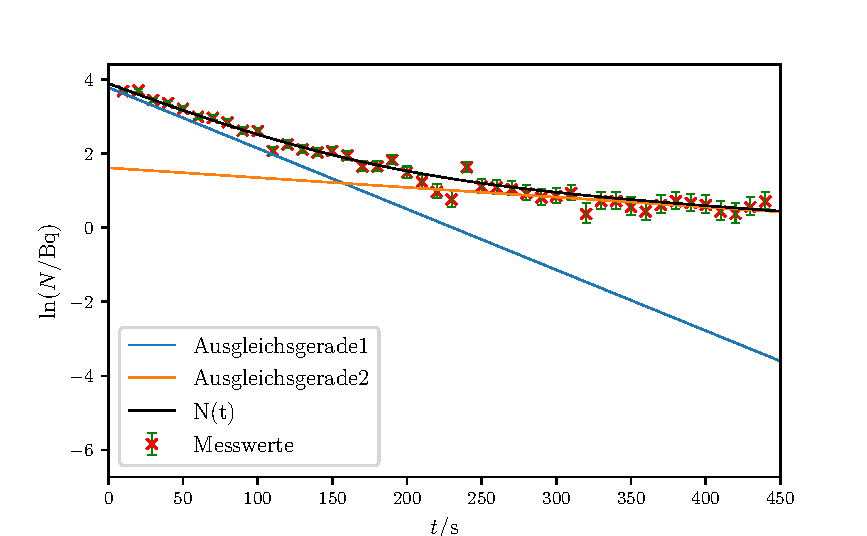
\includegraphics[width=\linewidth-50pt,height=\textheight-50pt,keepaspectratio]{content/images/RhodiumLog3.pdf}
	\caption{Die logarithmische Impulsrate $N_.{Rh}$ von Rhodium in Abhängigkeit von der Zeit $t$. Die erste Ausgleichsgerade ist nach Formel \eqref{eq:Ausgleich1}, die zweite nach Formel \eqref{eq:Ausgleich2} berechnet.}
	\label{fig:RhodiumLog3}
\end{figure}

\begin{figure}
	\centering
	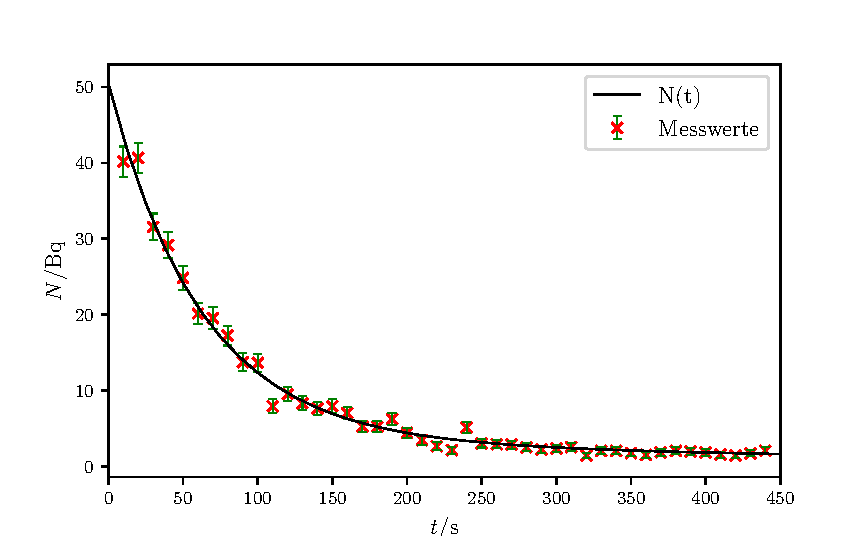
\includegraphics[width=\linewidth-50pt,height=\textheight-50pt,keepaspectratio]{content/images/Rhodium.pdf}
	\caption{Die Impulsrate $N_.{Rh}$ von Rhodium in Abhängigkeit von der Zeit $t$.}
	\label{fig:Rhodium}
\end{figure}
